\documentclass[a4paper,11pt]{article}
\usepackage[utf8]{inputenc}
\usepackage{minted}
\usepackage{amsmath}
\usepackage{float}
\usepackage{graphicx}
\usepackage[toc,page]{appendix}

\graphicspath{{./figures/}}

\title{\textbf{Stacks}}
\author{Kristiāns Vinters}
\date{Fall 2023}

\begin{document}
    \maketitle
    \section*{Introduction}

    I solved the stack/calculator assignment in Go. I used Go because I want to become more familiar with it. Source code and benchmark data is available on GitHub\footnote{https://github.com/Phanty133/id1021/tree/master/stack}.

    \section*{Implementation}

    I structured the program into three sub-packages: \texttt{solver}, \texttt{stacks}, \texttt{token}. The main function in \texttt{cmd/stack/main.go} only creates a stack from the \texttt{stacks} package and passes it and a string RPN expression to \texttt{solver.Solve()}.

    \subsection*{\texttt{stacks}}

    I utilize Go 1.18 generics to define generic stacks, but for the calculator I only allow a \texttt{float32} stack. The \texttt{stacks} package implements the \texttt{StaticStack} and \texttt{DynamicStack} and defines a \texttt{Stack} interface. The \texttt{Stack} interface defines generic stack methods, which are implemented by the specific stack structs.

    \begin{minted}{go}
type Stack[T any] interface {
    Push(val T) error
    Pop() (T, error)
    Empty() bool
}
    \end{minted}

Both stack structs are defined as follows with only the type name being different:
    \begin{minted}{go}
// or type DynamicStack[T any] struct { ...
type StaticStack[T any] struct {
    size int
    ip   int
    data []T
}
    \end{minted}

    For both stack types, most of the method functionality is shared. If the stack is not empty, the \texttt{Push} method increments the instruction pointer and sets the value at the pointer to the passed value. The \texttt{Pop} method returns the value at the internal pointer and decrements the pointer. If the user attempts to pop an empty stack, the method returns an underflow error. The \texttt{Empty} method returns true if the internal pointer is -1.

    \subsubsection*{\texttt{StaticStack}}

    A static stack is created with a constructor function, which expects a pre-defined fixed-length data array, because Go, as far as I am aware, does not support run-time fixed-length array allocation (run-time arrays are handled through slices). If the user attempts to push to a full stack, the \texttt{Push} method returns an overflow error.

    \begin{minted}{go}
func NewStaticStack[T any](dataArr []T) *StaticStack[T] {
    return &StaticStack[T]{
        size: cap(dataArr),
        ip:   -1,
        data: dataArr,
    }
}
    \end{minted}

    \subsubsection*{\texttt{DynamicStack}}

    A dynamic stack is created with a constructor function, which expects the initial size of the stack. The constructor allocates a slice of the specified size and returns a pointer to the stack struct. Although I use a slice, I perform under/overflow checks and reallocation manually.

    \begin{minted}{go}
func NewDynamicStack[T any](dataArr []T) *DynamicStack[T] {
    return &DynamicStack[T]{
        size: initialSize,
        ip:   -1,
        data: make([]T, initialSize),
    }
}
    \end{minted}

    To implement dynamic resizing, I defined a \texttt{Reallocate} method, which handles size changes and data copying:

    \begin{minted}{go}
func (stack *DynamicStack[T]) Reallocate(newSize int) {
    newData := make([]T, newSize)
    copy(newData, stack.data)
    stack.data = newData
    stack.size = newSize
}
    \end{minted}

    Whenever I push to the stack, I perform a check for whether the stack is full. If it is, I double the size:
    \begin{minted}{go}
if stack.ip == stack.size - 1 {
    stack.Reallocate(stack.size * 2)
}
    \end{minted}

    When I pop from the stack, I check whether the stack is less than a quarter full. If it is, I halve the size:
    \begin{minted}{go}
if stack.ip < stack.size / 4 {
    stack.Reallocate(stack.size / 2)
}
    \end{minted}

    I decided to do it this way to avoid frequent resizing. By checking for quarter capacity and resizing only by half, I leave a buffer which should handle most minor push/pops.

    \subsection*{\texttt{tokens}}
    
    The \texttt{token} package defines a \texttt{TokenType} enum for representing the operator type. The package also defines a token type-function map, which is used to map the operator type to the operator function.

    \begin{minted}{go}
var tokenFuncMap = map[TokenType]func(val1 float32, val2 float32) float32{
    ADD: func(val1 float32, val2 float32) float32 { return val1 + val2 },
    ...
}
    \end{minted}

    \subsection*{\texttt{solver}}

    The \texttt{solver} package contains calculator functions which use the other two packages. The calculator is structured around an \texttt{Expression} struct.
    
    \begin{minted}{go}
type Expression[StackType stacks.Stack[float32]] struct {
    numStack StackType
    ops []token.Token
}
    \end{minted}

    The package defines two internal \texttt{Expression} methods for parsing the string expression and solving it: \texttt{PopulateExpression} and \texttt{ParseExpression}. The  \texttt{PopulateExpression} takes in a normalized\footnote{All multi-spaces replaced with single spaces according to the regular expression \texttt{/\textbackslash s\{2,\}/}.} string expression and populates the value stack and operator array with values and operators, respectively.

    The \texttt{ParseExpression} method takes in a populated \texttt{Expression} and solves it. It iterates over the operator array and applies the operator function to the top two values in the value stack. The result is pushed back onto the value stack. The method returns the final value in the value stack.

    \section*{Stack benchmarks}

    To benchmark the stack implementations, I did 2000 runs, each of which consisted of a 1000 iterations of N pushes and N pops (sequentially as listed). The results for each run were then written to a CSV file. Code used for benchmarking is given in appendix \ref{appendix:benchmark_code}. I benchmarked both implementations for $\forall N\in\{100, 500, 1000, 2000, 5000\}$. Unsurprisingly, the static stack outperformed the dynamic stack in all cases, as per Fig. \ref{fig:median-times}. Results for all $N$ are given in appendix \ref{appendix:results}. The speedup ratio of static over dynamic doesn't appear to change significantly over $N$ (Fig. \ref{fig:ratio}), averaging out at about $1.5$.

    \begin{figure}[H]
        \centering
        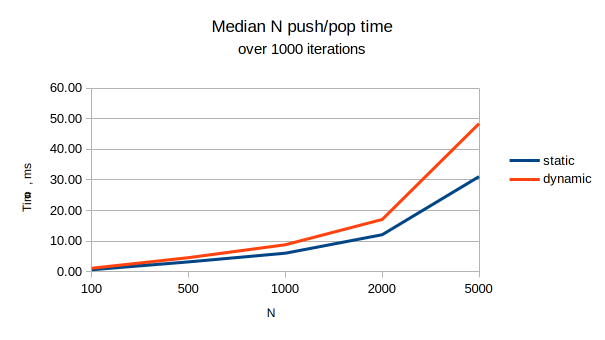
\includegraphics[width=0.9\textwidth]{median.png}
        \caption{Median times for both implementations}
        \label{fig:median-times}
    \end{figure}

    \begin{figure}[H]
        \centering
        \begin{tabular}{c|c}
            N & Speedup ratio \\
            \hline
            \hline
            100 & 1.8 \\
            \hline
            500 & 1.4 \\
            \hline
            1000 & 1.5 \\
            \hline
            2000 & 1.4 \\
            \hline
            5000 & 1.6 \\
        \end{tabular}
        \caption{$Ratio = \frac{Med(DynamicTimes)}{Med(StaticTimes)}$}
        \label{fig:ratio}
    \end{figure}

    An interesting observation is that the static stack run times are more consistent than the dynamic stack run times for all $N$. This is evident in the run time histograms (Fig. \ref{fig:histo1000}). The static stack times are more consistent most likely because the stack is pre-allocated and the run time is not affected by the size of the stack. On the other hand, the dynamic stack times are more inconsistent because the stack is dynamically reallocated, thus likely more susceptible to background processes.

    \begin{figure}[H]
        \centering
        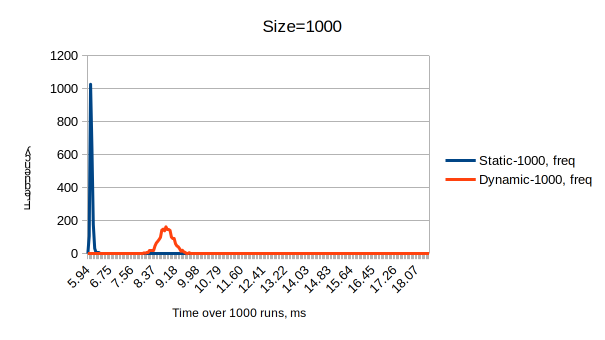
\includegraphics[width=0.9\textwidth]{size1000histo.png}
        \caption{N=1000 run time histogram, all $N$ histograms in appendix \ref{appendix:histos}}
        \label{fig:histo1000}
    \end{figure}

    \begin{appendices}
        \section{Benchmark code}
        \label{appendix:benchmark_code}

        \begin{minted}{go}
func StackBench[StackType stacks.Stack[int]](
    tag string,
    stack StackType,
    runs int,
    runIters int,
    stackIters int
) {
    outFile, err := os.Create(fmt.Sprintf("stack_%s.csv", tag))

    if err != nil {
        fmt.Println(err)
        return
    }

    defer outFile.Close()

    runTimes := make([]time.Duration, runs)

    for run := 0; run < runs; run++ {
        runStart := time.Now()

        for iter := 0; iter < runIters; iter++ {
            for i := 0; i < stackIters; i++ {
                stack.Push(i)
            }
    
            for i := 0; i < stackIters; i++ {
                stack.Pop()
            }
        }

        runTimes[run] = time.Since(runStart)
    }

    writer := csv.NewWriter(outFile)
    defer writer.Flush()

    for _, time := range runTimes {
        writer.Write([]string{fmt.Sprintf("%d", time.Microseconds())})
    }
}
        \end{minted}

        \section{Benchmark results}
        \label{appendix:results}

        \begin{figure}[H]
            \centering
            \begin{tabular}{c|c|c|c|c|c}
                Impl. & Min, ms & Max, ms & Mean, ms & Median, ms & Std.dev, ms \\
                \hline
                \hline
                Static & 0.60 & 0.91 & 0.62 & 0.62 & 0.01 \\
                \hline
                Dynamic & 0.9 & 2.7 & 1.1 & 1.1 & 0.16 \\
            \end{tabular}
            \caption{N=100}
        \end{figure}
        \begin{figure}[H]
            \centering
            \begin{tabular}{c|c|c|c|c|c}
                Impl. & Min, ms & Max, ms & Mean, ms & Median, ms & Std.dev, ms \\
                \hline
                \hline
                Static & 3.02 & 5.17 & 3.20 & 3.20 & 0.14 \\
                \hline
                Dynamic & 4.0 & 6.6 & 4.6 & 4.6 & 0.24 \\
            \end{tabular}
            \caption{Results for N=500}
        \end{figure}
        \begin{figure}[H]
            \centering
            \begin{tabular}{c|c|c|c|c|c}
                Impl. & Min, ms & Max, ms & Mean, ms & Median, ms & Std.dev, ms \\
                \hline
                \hline
                Static & 5.94 & 7.28 & 6.05 & 6.04 & 0.07 \\
                \hline
                Dynamic & 8.0 & 18.6 & 8.8 & 8.8 & 0.38 \\
            \end{tabular}
            \caption{N=1000}
        \end{figure}
        \begin{figure}[H]
            \centering
            \begin{tabular}{c|c|c|c|c|c}
                Impl. & Min, ms & Max, ms & Mean, ms & Median, ms & Std.dev, ms \\
                \hline
                \hline
                Static & 11.95 & 15.43 & 12.18 & 12.08 & 0.26 \\
                \hline
                Dynamic & 15.8 & 21.8 & 17.1 & 17.1 & 0.46 \\
            \end{tabular}
            \caption{N=2000}
        \end{figure}
        \begin{figure}[H]
            \centering
            \begin{tabular}{c|c|c|c|c|c}
                Impl. & Min, ms & Max, ms & Mean, ms & Median, ms & Std.dev, ms \\
                \hline
                \hline
                Static & 30.14 & 52.54 & 31.55 & 31.08 & 1.87 \\
                \hline
                Dynamic & 45.4 & 75.5 & 50.3 & 48.4 & 4.08 \\
            \end{tabular}
            \caption{N=5000}
        \end{figure}

        \section{Run time histograms}
        \label{appendix:histos}

        \begin{figure}[H]
            \centering
            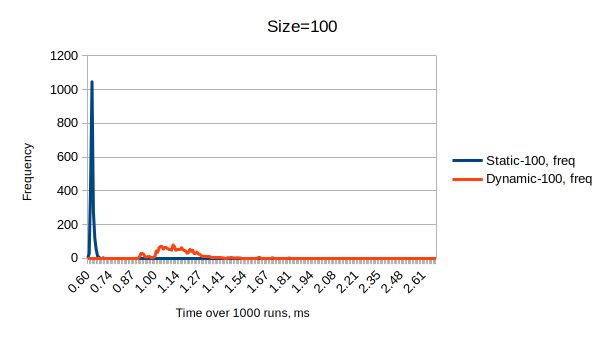
\includegraphics[width=0.9\textwidth]{size100histo.png}
            \caption{N=100}
        \end{figure}
        \begin{figure}[H]
            \centering
            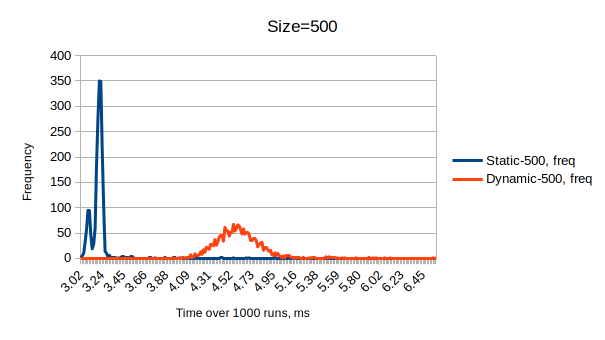
\includegraphics[width=0.9\textwidth]{size500histo.png}
            \caption{N=500}
        \end{figure}
        \begin{figure}[H]
            \centering
            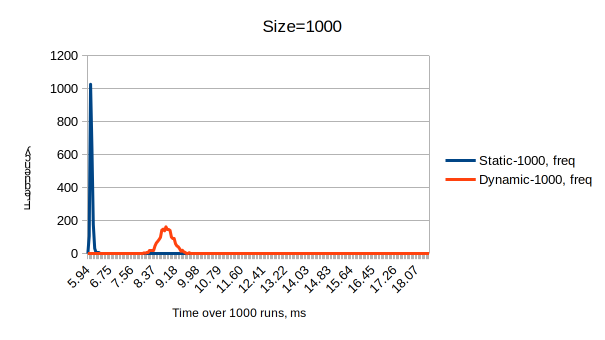
\includegraphics[width=0.9\textwidth]{size1000histo.png}
            \caption{N=1000}
        \end{figure}
        \begin{figure}[H]
            \centering
            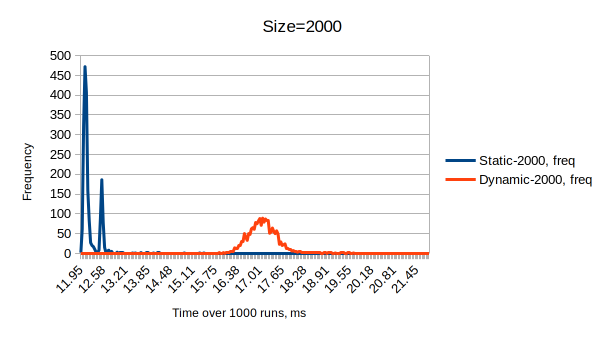
\includegraphics[width=0.9\textwidth]{size2000histo.png}
            \caption{N=2000}
        \end{figure}
        \begin{figure}[H]
            \centering
            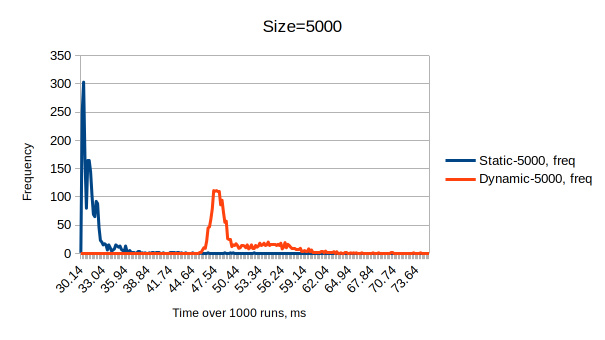
\includegraphics[width=0.9\textwidth]{size5000histo.png}
            \caption{N=5000}
        \end{figure}
    \end{appendices}
\end{document}
